%%%%%%%%%%%%%%%%%%%%%%%%%%%%%%%%%%%%%%%%%%%%%%%%%%%%%%%%%%%%%%%%%%%%%%%%%%%%%%%%%%%%%%%%%%%%%%%%%
%
% Document:     Data Management  product tree
%
%%%%%%%%%%%%%%%%%%%%%%%%%%%%%%%%%%%%%%%%%%%%%%%%%%%%%%%%%%%%%%%%%%%%%%%%%%%%%%
\documentclass{article}
\usepackage{times,layouts}
\usepackage{tikz,hyperref,amsmath}
\usetikzlibrary{positioning,arrows,shapes,decorations.shapes,shapes.arrows}
\usetikzlibrary{backgrounds,calc}
\usepackage[paperwidth=62.400000000000006cm,paperheight=16.1cm,
left=-2mm,top=3mm,bottom=0mm,right=0mm,
noheadfoot,marginparwidth=0pt,includemp=false,
textwidth=30cm,textheight=50mm]{geometry}
\newcommand\showpage{%
\setlayoutscale{0.5}\setlabelfont{\tiny}\printheadingsfalse\printparametersfalse
\currentpage\pagedesign}
\hypersetup{pdftitle={DM products }, pdfsubject={Diagram illustrating the
                products in LSST DM }, pdfauthor={Autogenerated from MD}}
\tikzstyle{tbox}=[rectangle,text centered, text width=30mm]
\tikzstyle{wbbox}=[rectangle, rounded corners=3pt, draw=black, top color=blue!50!white,
                    bottom color=white, very thick, minimum height=12mm, inner sep=2pt,
                    text centered, text width=30mm]
\tikzstyle{pbox}=[rectangle, rounded corners=3pt, draw=black, top
 color=yellow!50!white, bottom color=white, very thick,
 minimum height=35pt, inner sep=2pt, text centered, text width=35mm]
\tikzstyle{pline}=[-, thick]
\begin{document}
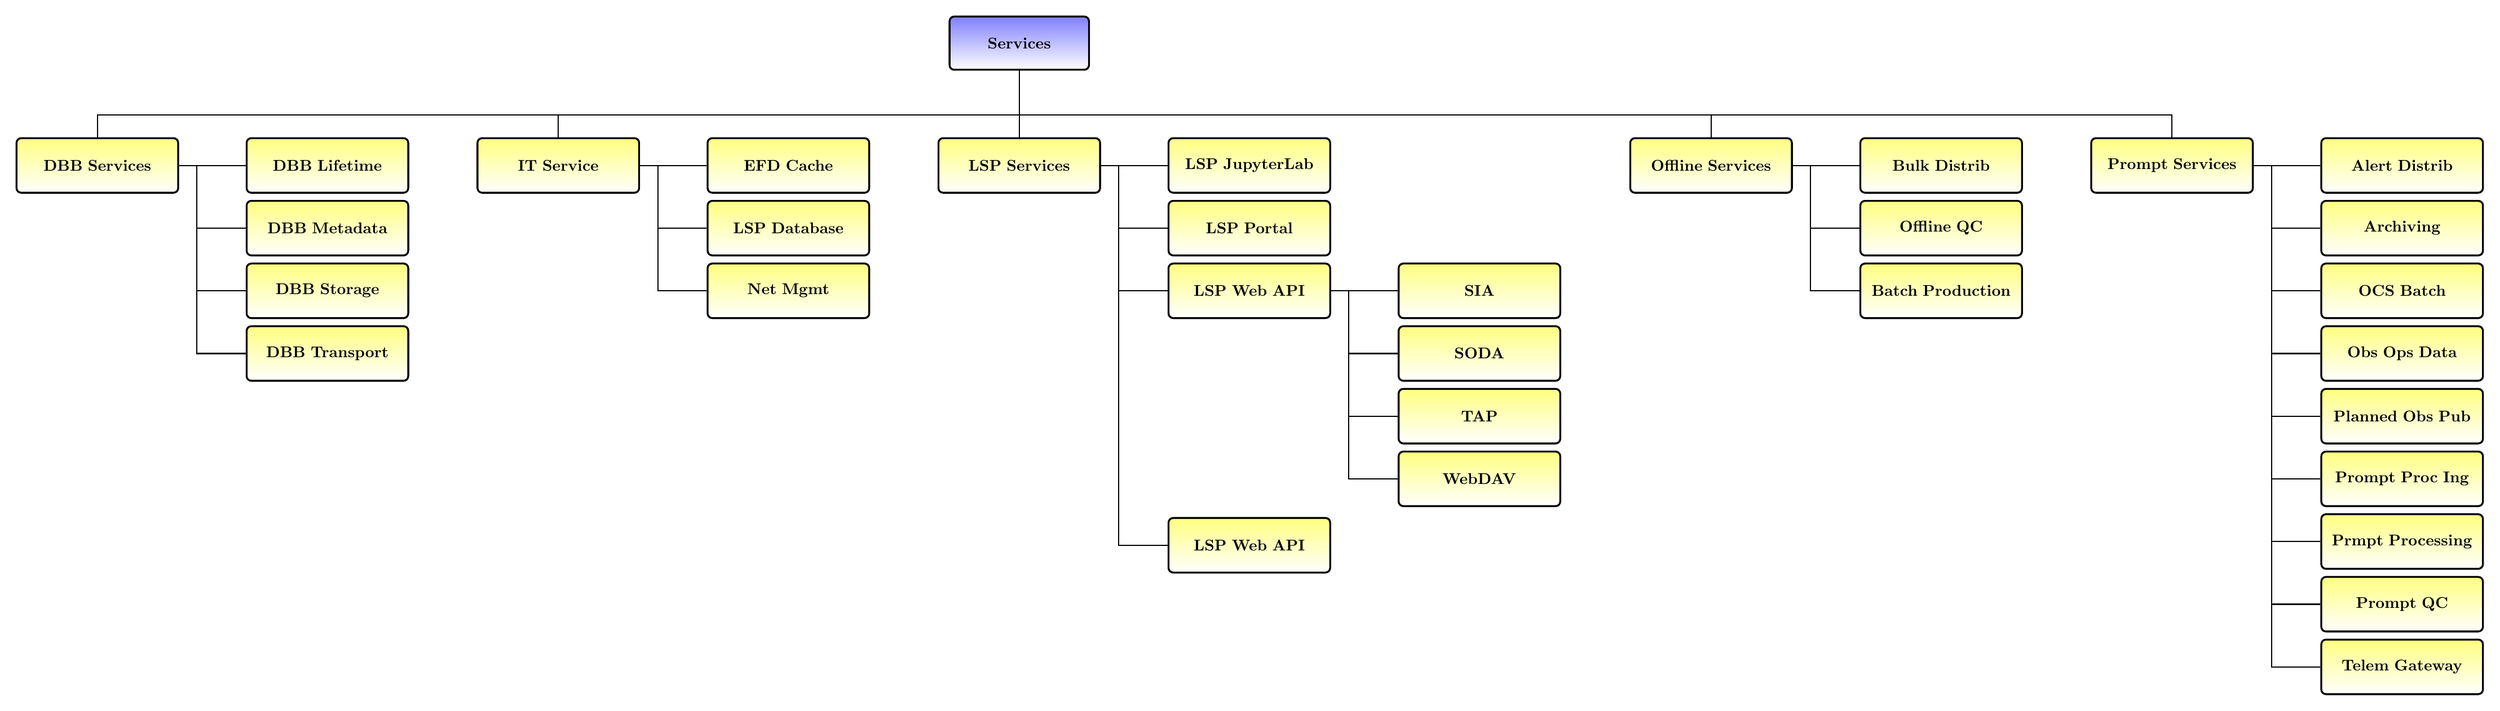
\begin{tikzpicture}[node distance=0mm]


\node (DBBSRV) [pbox, 
] {\textbf{DBB Services
} };
\node (DBBLIFESRV) [pbox,right=15mm of DBBSRV] {\textbf{DBB Lifetime
} };
 \draw[pline] (DBBSRV.east) -| ++(0.4,0) |- (DBBLIFESRV.west); 
\node (DBBMDSRV) [pbox,below=4pt of DBBLIFESRV] {\textbf{DBB Metadata
} };
 \draw[pline] (DBBSRV.east) -| ++(0.4,0) |- (DBBMDSRV.west); 
\node (DBBSTRSRV) [pbox,below=4pt of DBBMDSRV] {\textbf{DBB Storage
} };
 \draw[pline] (DBBSRV.east) -| ++(0.4,0) |- (DBBSTRSRV.west); 
\node (DBBTRSRV) [pbox,below=4pt of DBBSTRSRV] {\textbf{DBB Transport
} };
 \draw[pline] (DBBSRV.east) -| ++(0.4,0) |- (DBBTRSRV.west); 
\node (ITSRV) [pbox, 
right=6.7cm of DBBSRV] {\textbf{IT Service
} };
\node (EFDB) [pbox,right=15mm of ITSRV] {\textbf{EFD Cache
} };
 \draw[pline] (ITSRV.east) -| ++(0.4,0) |- (EFDB.west); 
\node (LSPDB) [pbox,below=4pt of EFDB] {\textbf{LSP Database
} };
 \draw[pline] (ITSRV.east) -| ++(0.4,0) |- (LSPDB.west); 
\node (NETMGMT) [pbox,below=4pt of LSPDB] {\textbf{Net Mgmt
} };
 \draw[pline] (ITSRV.east) -| ++(0.4,0) |- (NETMGMT.west); 
\node (LSPSRV) [pbox, 
right=6.7cm of ITSRV] {\textbf{LSP Services
} };
\node (LSPJLSRV) [pbox,right=15mm of LSPSRV] {\textbf{LSP JupyterLab
} };
 \draw[pline] (LSPSRV.east) -| ++(0.4,0) |- (LSPJLSRV.west); 
\node (LSPPRTLSRV) [pbox,below=4pt of LSPJLSRV] {\textbf{LSP Portal
} };
 \draw[pline] (LSPSRV.east) -| ++(0.4,0) |- (LSPPRTLSRV.west); 
\node (LSPWAPI) [pbox,below=4pt of LSPPRTLSRV] {\textbf{LSP Web API
} };
 \draw[pline] (LSPSRV.east) -| ++(0.4,0) |- (LSPWAPI.west); 
\node (SIASRV) [pbox,right=15mm of LSPWAPI] {\textbf{SIA
} };
 \draw[pline] (LSPWAPI.east) -| ++(0.4,0) |- (SIASRV.west); 
\node (SODA) [pbox,below=4pt of SIASRV] {\textbf{SODA
} };
 \draw[pline] (LSPWAPI.east) -| ++(0.4,0) |- (SODA.west); 
\node (TAPSEV) [pbox,below=4pt of SODA] {\textbf{TAP
} };
 \draw[pline] (LSPWAPI.east) -| ++(0.4,0) |- (TAPSEV.west); 
\node (WDAV) [pbox,below=4pt of TAPSEV] {\textbf{WebDAV
} };
 \draw[pline] (LSPWAPI.east) -| ++(0.4,0) |- (WDAV.west); 
\node (LSPWEBSRV) [pbox,below=127pt of LSPWAPI] {\textbf{LSP Web API
} };
 \draw[pline] (LSPSRV.east) -| ++(0.4,0) |- (LSPWEBSRV.west); 
\node (OFFLSRV) [pbox, 
right=11.9cm of LSPSRV] {\textbf{Offline Services
} };
\node (BULKDSRV) [pbox,right=15mm of OFFLSRV] {\textbf{Bulk Distrib
} };
 \draw[pline] (OFFLSRV.east) -| ++(0.4,0) |- (BULKDSRV.west); 
\node (OFFLQCSRV) [pbox,below=4pt of BULKDSRV] {\textbf{Offline QC
} };
 \draw[pline] (OFFLSRV.east) -| ++(0.4,0) |- (OFFLQCSRV.west); 
\node (PRODSRV) [pbox,below=4pt of OFFLQCSRV] {\textbf{Batch Production
} };
 \draw[pline] (OFFLSRV.east) -| ++(0.4,0) |- (PRODSRV.west); 
\node (PRSRV) [pbox, 
right=6.7cm of OFFLSRV] {\textbf{Prompt Services
} };
\node (ALRTDSTSRV) [pbox,right=15mm of PRSRV] {\textbf{Alert Distrib
} };
 \draw[pline] (PRSRV.east) -| ++(0.4,0) |- (ALRTDSTSRV.west); 
\node (ARCSRV) [pbox,below=4pt of ALRTDSTSRV] {\textbf{Archiving
} };
 \draw[pline] (PRSRV.east) -| ++(0.4,0) |- (ARCSRV.west); 
\node (OCSBATSRV) [pbox,below=4pt of ARCSRV] {\textbf{OCS Batch
} };
 \draw[pline] (PRSRV.east) -| ++(0.4,0) |- (OCSBATSRV.west); 
\node (OODSSRV) [pbox,below=4pt of OCSBATSRV] {\textbf{Obs Ops Data
} };
 \draw[pline] (PRSRV.east) -| ++(0.4,0) |- (OODSSRV.west); 
\node (POPSRV) [pbox,below=4pt of OODSSRV] {\textbf{Planned Obs Pub
} };
 \draw[pline] (PRSRV.east) -| ++(0.4,0) |- (POPSRV.west); 
\node (PRPINGSRV) [pbox,below=4pt of POPSRV] {\textbf{Prompt Proc Ing
} };
 \draw[pline] (PRSRV.east) -| ++(0.4,0) |- (PRPINGSRV.west); 
\node (PRPRSRV) [pbox,below=4pt of PRPINGSRV] {\textbf{Prmpt Processing
} };
 \draw[pline] (PRSRV.east) -| ++(0.4,0) |- (PRPRSRV.west); 
\node (PRQCSRV) [pbox,below=4pt of PRPRSRV] {\textbf{Prompt QC
} };
 \draw[pline] (PRSRV.east) -| ++(0.4,0) |- (PRQCSRV.west); 
\node (TMGSRV) [pbox,below=4pt of PRQCSRV] {\textbf{Telem Gateway
} };
 \draw[pline] (PRSRV.east) -| ++(0.4,0) |- (TMGSRV.west); 
\node (DMSRV) [wbbox, above=15mm of LSPSRV]{\textbf{Services
}};
 \draw[pline]   (DBBSRV.north) -- ++(0.0,0.5) -| (DMSRV.south) ; 
 \draw[pline]   (ITSRV.north) -- ++(0.0,0.5) -| (DMSRV.south) ; 
 \draw[pline]   (LSPSRV.north) -- ++(0.0,0.5) -| (DMSRV.south) ; 
 \draw[pline]   (OFFLSRV.north) -- ++(0.0,0.5) -| (DMSRV.south) ; 
 \draw[pline]   (PRSRV.north) -- ++(0.0,0.5) -| (DMSRV.south) ; 

\end{tikzpicture}
\end{document}
